\documentclass[english,12pt]{article}

\usepackage{sbc-template}

\usepackage{graphicx,color,url}
\usepackage{subfigure}                  % Subfiguras
\usepackage{epsfig}         % tratamento de figuras EPS

  
%\usepackage[brazil]{babel}   
\usepackage[latin1]{inputenc}  
        
\sloppy 

\title{Non-Functional Requirements for Service-Based Applications: A Systematic Review}

\author{Pl\'acido A. Souza Neto\inst{1} \and Martin A. Musicante\inst{2}\\ 
Genoveva Vargas-Solar\inst{3} \and Valeria de Castro\inst{4}\\
Umberto Souza da Costa\inst{2} }
 
 
\address{ 
Instituto Federal do Rio Grande do Norte\\ 
Campus Natal-Central -- RN - Brazil
\nextinstitute
DIMAp - Universidade Federal do Rio Grande do Norte\\
Campus Universit\'ario -- Natal -- RN -- Brazil
\nextinstitute
Universit\'e de Grenoble\\
Saint Martin d'H\`{e}res -- France
\nextinstitute
Universidad Rey Juan Carlos\\
M\'{o}stoles -- Spain
\email{placido.neto@ifrn.edu.br, \{umberto, mam\}@dimap.ufrn.br}\\
\email{genoveva.vargas-solar@imag.fr, valeria.decastro@urjc.es}
}
 

\begin{document} 
 
\maketitle
 
\begin{abstract}
 This paper presents a systematic literature review of non-functional
requirements (NFRs) for service-based applications. 
The main goal of the review is to identify the most common terms used to refer to NFRs.
We also propose a classification of the most common terms, as well as, a model to integrate those terms.
 
\end{abstract}


\section{Introduction}

Functional properties of a computer system are characterized by the effect produced by the system when given a defined input.
Functional properties are not the only crucial aspect in the software development process. 
Other properties need to be addressed to fit in the application with its context.
These other aspects are called Non-Functional Properties.

Non-Functional Requirements (NFRs) specify those properties that are not addressed by the functional  specification.
They are often called \textit{qualities} of the software system.
%They are also referred as ``constraints'', ``quality attributes'', ``quality goals'', ``quality of
%service requirements'' and ``non-behavioural requirements'' \cite{Stellman2005}.
Non-Functional Requirements may specify response time, security constraints or quality of the solution, among others.




Service-Oriented Computing~\cite{Papazoglou2007}, is a software development paradigm where pre-existing services are combined to produce more complex applications. 
%The selection of services is usually guided by the functional requirements of the application. 
%In this scenario, there exists the need to provide support for the specification of non-functional requirements, such as
%security, reliability, and efficiency. 
The development of service-based applications can benefit from the inclusion of NFRs to the software process from its early stages.
Failure to comply with this inclusion means that the final application is obtained from a partial specification, making the deployment a difficult task.
%Ideally, non-functional requirements
%would be considered along with all the stages of the software development. 
The adoption of non-functional specifications from the early states of development
can help the developer to produce applications that are capable of dealing with
their context.
Non-functional properties of service oriented applications have been
addressed in academic works and standards~\cite{ws-co,ws-tra,wsci}.
Different proposals~\cite{Babamir2010,AgarwalLS09,CholletL09,GutierrezRF10,XiaoCZBOLH08,JeongCL09,TsadimasNA12}
support non-functional requirements in the context of web service development. 

Most software development methods define software processes that use the notion of refinement.
Software process begins with the formulation of an abstract specification, which is successively refined to yield the implementation of the system.
Methods for the development of web service applications are no exception to this rule.
At least two levels of abstraction can be distinguished: a \textit{Business Level}, including the abstract specification, and a \textit{System Level}, including actual computer programs that implements the system.

In the case of web service applications we will distinguish two separate layers of the implementation.
The \textit{Composition Layer} is the upper layer of the implementation. 
It defines the workflow of the system, in terms of individual service calls.
The \textit{Service Layer} defines those services that are called by the composition.

\bigskip
 
In this work we investigate the extent in which NFRs are considered by the development methods proposed in the literature.
We have conducted a systematic review~\cite{Kitchenham08} to summarize the approaches that support NFRs.
As a result, we propose a classification of NFRs for web services.

\bigskip

This paper is organized as follows: 
Section~\ref{sec:sr} presents a systematic literature review of non-functional requirements for service-based applications.
The findings of the systematic review are presented in Section~\ref{sec:nfindings} and used in Section~\ref{sec:classification} to propose a classification and a model for NFRs in the context of web service development. 
Section~\ref{sec:conclusion} concludes the paper.


\section{A Systematic Review}  
\label{sec:sr}

In this work we develop a systematic literature review of NFRs for web services. 
Our review considers the abstraction levels and implementation layers defined above. 
%
%We present a systematic review of the non-func\-tion\-al
%requirements and properties used in the context of service-oriented
%development. 
The purpose of our analysis is to: 
\textit{(i)} Identify concepts, properties and notations related to NFRs and used in service-based system development; and 
\textit{(ii)} Define a classification for these concepts, properties and notations, at different  levels of abstraction.

%For each phase of the software process, the requirements and non-functional
%requirements are refined. 
%As a result of this process, the granularity of the
%concepts described by the requirement becomes thinner and more precise. 

% The focus of a modeling-based non-functional requirements becomes important
% because it reveals a continuing need on the development of distributed
% service-oriented. Thus, it is necessary identify how non-functional requirements
% are classified in different development process phases and iterations.

% Thus, this section also presents the collected data and results
% from the research work analysis according to some research questions. Once the
% sources' extraction execution had been completed, it was important to be sure
% that multiple publications of the same approach were not included in the data analysis. Tables \ref{tab:result02}
% and \ref{tab:result03} show the results of each work under each question
% described in section \ref{subsec:question}.  





% % Among the properties presented we highlight the security
% % and performance properties. All users want to access data
% % securely and quickly. Most studies analyzed have both properties. Reliability is
% % also an important non-functional requirement presented in some papers and needed
% % to end users. 

% 
% The analisys was carried out by effectuating the following activities:
% \textit{(i) question formulation; (ii) source selection; (iii) selection
% process; (iv) information extraction;} and \textit{(v) results}.

We propose seven research questions ($RQ_1$ to $RQ_7$) to guide our analysis about non-functional
requirements for web services. 
For each question we define a set of possible answers in order to guide
the analysis.
%These possible answers are defined from our knowledge on each topic. 
The questions are:
\begin{itemize} 
  \item \textbf{\texttt{$RQ_1$:}} How NFRs are modelled by existing
  methodologies for Web services?
  %\begin{trivlist}
%	  \item 
Possible answers: \textit{Answer is specific to each proposal.}
	%\end{trivlist}  
 \item \textbf{\texttt{$RQ_2$:}} Which kinds of NFRs are considered more frequently?
 	%\begin{trivlist}
	  %\item 
	  Possible answers: \textit{Security / availability / portability / \ldots / reliability /
	  performance.}
	%\end{trivlist}
  \item \textbf{\texttt{$RQ_3$:}} What is the main underlying approach used by the proposal?
	%\begin{trivlist}
%	  \item 
Possible answers: \textit{Model driven approach (MDD) / Ontologies (Ont) / Formal methods (FM) / Artificial intelligence (AI) / Business Process Modeling (BP) / Traditional (TDT).}
	%\end{trivlist} 
  \item \textbf{\texttt{$RQ_4$:}} What is the scope of the proposal?
  %\begin{trivlist}
%	  \item 
Possible answers: \textit{Software architecture / QoS model / Language definition / Methodology / etc.}
	%\end{trivlist}	
  \item \textbf{\texttt{$RQ_5$:}} Does the paper propose a (meta)model
  for NFRs? Does the Business Level specification include NFRs?  
%\begin{trivlist}
%	  \item 
Possible answers: \textit{yes / no} -- \textit{yes / no.}
%	\end{trivlist}  
  \item \textbf{\texttt{$RQ_6$:}} Are non-functional aspects considered at the composition or single service level?
%\begin{trivlist}
%	  \item 
Possible answers: \textit{single / composition.}
%	\end{trivlist}
\item \textbf{\texttt{$RQ_7$:}} What is the publication year of the paper?
%	\begin{trivlist}
%	  \item 
Possible answers: \textit{Year of publication.}
%	\end{trivlist}	   
\end{itemize}


We use the approach described in~\cite{Kitchenham08} for searching,
collecting and selecting works related with NFRs for service-based applications. 
The results are used to identify and compare key concepts related to NFRs.
The search engines used in our review include journals, conferences and
workshops of recognized quality. 
We used the following search engines: \textit{(i) IEEE Computer; (ii) ACM Digital Library;} and
\textit{(iii) Science Direct}.

The query used to perform the search is defined as: 
 \begin{center}
\texttt{(((non functional properties) OR (non functional requirements))
AND web service AND composition))}
\end{center}

The results of our query for each search engine were filtered in accordance to the following criteria:
\begin{enumerate}
\item[1.] Papers written in other languages than English were excluded.
\item[2.] Papers published in non-international conferences and workshops were also excluded.
\item[3.] Papers whose title and abstract do not refer to NFRs were excluded. 
\end{enumerate}

After this filtering process, the remaining papers were analyzed in full.
A brief account of our findings is given in the next section.

\section{Our Findings}   
\label{sec:nfindings}   




In this section we analyze the results of the search query for our systematic review.
The search was performed on three different scientific sources, namely IEEE Computer, ACM Digital Library (only journal papers) and Science Direct.
We first show the contribution of each search engine, in terms of the number of relevant papers and year of publication.
Next, we summarize the answers we have obtained to the questions of our systematic review.


\begin{table}[ht!]
\small
\centering
\begin{tabular}{l|c|c|c|c}
  \hline
  \hline
   & IEEE & ACM  & Science Direct & Total \\
  \hline
  \hline
  Total  & 76 &  88  & 248 & 412 \\
  \hline
  Title/Abstract & 25 (32.9\%) & 12 (13.6\%) & 30 (12.1\%)  & 67 (16.3\%) \\
  \hline
  Full text & 11 (14.5\%) & 3 (3.4\%) & 12 (4.8\%) & 26 (6.3\%)\\
  \hline
  \hline
\end{tabular}
\caption{Number of papers per source.}
\label{tab:result01}
\end{table}
 

Table \ref{tab:result01} shows the number of papers obtained at each stage
of the selection procedure, for each source. 
The first row shows the total number of papers returned by each engine, for the search query (Section~\ref{sec:sr}).
The next row of the table shows the results obtained after filtering the papers by considering their titles and abstracts.
The percentage figures indicate the proportion of remaining papers, for each source.
The last row of the table shows the number of relevant papers obtained, after considering the complete text of each paper.
The percentages are relative to the total, for each source.
The distribution of publication year for the 26 selected papers is shown in Figure~\ref{fig:statistics}.


\begin{figure} 
\centering
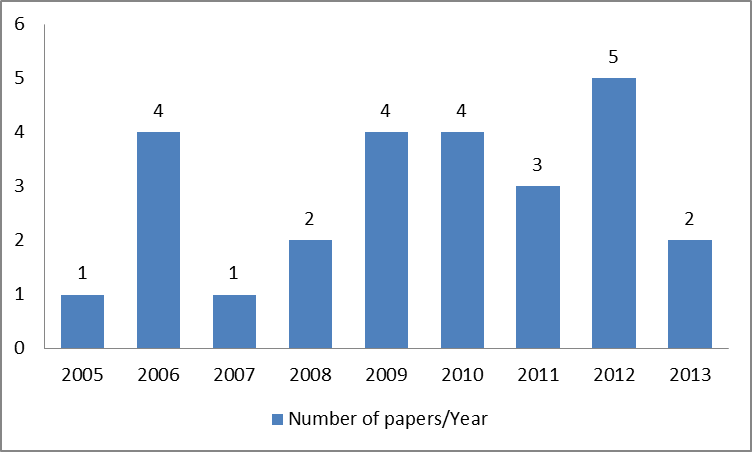
\includegraphics[width=.79\textwidth]{figs/NumberPapersYear.png}
\caption{Publications per year.}
\label{fig:statistics}
\end{figure}

For each of the 26 papers, we obtained answers for each research question.
Our findings are presented in Tables~\ref{tab:result02} and~\ref{tab:result03}.

  
\begin{table*}[ht!]
\centering
%\scriptsize
%\tiny
\small
\begin{tabular}{l|l|l|l|l}
  \hline 
  \hline
   \textbf{Reference}    & \textbf{$RQ_1$} &
   \textbf{$RQ_2$} & \textbf{$RQ_3$} &
   \textbf{$RQ_4$} 
   \\
                    & \textbf{\textit{NFR concepts}} &
   \textbf{\textit{Properties}} & \textbf{\textit{Approach}} &
   \textbf{\textit{Domain / Scope}} 
   \\
  \hline
  \hline  
  Babamir et al. \cite{Babamir2010} &  property / & responsiveness / & TDT & Software  \\
                                                       & category /  & availability           &         & architecture \\
                                                       & constraint  & performance        &         &  \\
                                                       &                  & / sla properties    &         &  \\  
  \hline   
  Yeom et al. \cite{Yeom2006}         & category /                    & business value /                   & TDT & QoS model\\ 
                                                       & sub-category /             & performance /                      &        &                  \\
                                                       & property                       & stability /                             &        &                  \\
                                                       &                                     & manageability /                    &        &                  \\
                                                       &                                     & security /                              &        &                  \\
                                                       &                                     & business                               &         &                  \\
                                                      &                                     &  processing                           &         &                  \\
                                                      &                                      & interoperability                     &        &                  \\ 
  \hline 
  Xiao et al. \cite{XiaoCZBOLH08} &  NF attribute  & time / cost /   & BP  & Business processes   \\   
                                                    &                      & resource         &       &  modelling \\
  \hline 
  D'Ambrogio \cite{DAmbrogio06} &  characteristics /  & availability /                & MDD & WSDL extension \\
                                                     & category /            & reliability /                  &         &  \\
                                                     & dimension            & access control             &         &  \\
   \hline
  Chollet et al. \cite{CholletL09} & activity /             & security  & MDD  & Orchestration   \\
                                                  & NF attribute        &              &            &   Framework  \\
  \hline
  Schmeling et al. \cite{SchmelingCM11} & NF concern /      & security &  MDD &  Web service  \\
                                                               & NF attribute /    &               &          &  composition              \\
                                                               & NF action /        &               &          &   process         \\
                                                               & NF activity         &               &          &   \\ 
  \hline
    Thi{\ss}en et al. \cite{ThissenW06} & NF value  & performance /   &  FM & Software  \\  
                                                          &                & reliability /         &       &   architecture        \\
                                                          &                & cost /                 &        &            \\
                                                          &                & availability &  & \\  
  \hline
  Zhang et al. \cite{ZhangPSP05} & attribute / & security & FM &  Access control   \\
                                                   & predicate  &              &       &               \\
  \hline
  Basin et al. \cite{BasinDL06} &  attribute & security  & MDD & System \\
                                              &                &               &          &   architecture
  \\
  \hline
  Ceri et al. \cite{CeriDMF07} & policy / rule / & n.a. & TDT & Context-aware    \\
                                              & condition /    &        &        & applications     \\
                                              &  action           &         &       &          
  \\
  \hline
  Fabra et al. \cite{Fabra2011} & property & storage /     & MDD & Web service   \\
                                               &                & processing &          & methodology  \\
  \hline
  Modica et al. \cite{ModicaTV09} & quality level & sla properties & TDT &  Service oriented \\
                                                    &                    &                        &         & architecture  \\
  \hline
  Ovaska et al. \cite{OvaskaEHPA10} & attribute /  & security /    & MDD &  Model  \\
                                                        & category     & reliability    &          &   development                  \\
  \hline
  Agarwa et al. \cite{AgarwalLS09} & property /   & \textit{not explicitly}  & Ont & Policy language  \\
                                                     & policy /       & \textit{defined}          &        &                     \\
                                                     & function      &                                   &        &                \\
  \hline
  \hline  
\end{tabular} 
\caption{Research question results - $RQ_1$, $RQ_2$, $RQ_3$, $RQ_4$.}
\label{tab:result02a}
\end{table*} 

\begin{table*}[ht!]
\centering
\scriptsize
%\tiny
%\small
\begin{tabular}{l|l|l|c|l}
  \hline 
  \hline
   \textbf{Reference} & \textbf{$RQ_1$:\textit{NFR concepts}} &
   \textbf{$RQ_2$:\textit{Properties}} & \textbf{$RQ_3$:\textit{Approach}} &
   \textbf{$RQ_4$:\textit{Domain / Scope}} 
   \\
  \hline
  \hline  
   Jeong et al. \cite{JeongCL09} & NF attribute     & operation cost / & AI & Service oriented  \\
                                               &                         & performance /   &    &        architecture         \\
                                               &                         & availability /       &    &                                   \\
                                               &                         & accessibility /     &    &                                   \\
                                               &                         & security /            &    &                                   \\
                                               &                         & interoperability / &    &                                   \\
                                               &                         & usability /            &    &                                   \\
                                               &                         & user satisfaction & & \\
  \hline
 Pastrana et al. \cite{PastranaPK11}  & NF property / contract  / & performance / reliability / scalability / & Ont & Web service methodology\\
   &assertion / NF behaviour &  capacity / robustness / precision / security /&  & \\
  &  & accessibility / availability / interoperability    &  & \\    
  \hline
  Diamadopoulou et al. \cite{DiamadopoulouMPS08} & NF characteristic &
  user' subjective perception & TDT & Web service selection  \\ 
  \hline
  Gutierrez et al. \cite{GutierrezRF10} & NF factor / NF sub-factor & Security  & BP &  WS development process
  \\  
  \hline
  Mohanty et al. \cite{MohantyRP10} & NF attribute / NF factor & reliability /
  performance / integrity / & AI & Artificial intelligence /\\ 
  &  &  usability / response time / documentation &   & Web services classification	 \\
  \hline  
   Karunamurthy et al. \cite{Karunamurthy2012787} & Non-functional parameters &
   cost / response time / availability /  security /   & BP &  DSL (NFSL)
\\
   &  & availability / reliability / reputation   &  & 
  \\  
  \hline  
   Liu et al. \cite{Liu20121080} & QoS parameter &
   cost / execution duration / accuracy /  & FM  &  QoS model
\\
   &  &  security / integrity / availability / reliability   &   & 
  \\
  \hline 
 
   Tran et al. \cite{Tran2012531} & QoS policies &
   performance / availability / security /  & MDD  &  Language definition /
\\
   &  &  response time /  SLA aspects  &   &  QoS model
  \\  
  \hline   

 
   Wang et al. \cite{Wang2012} & Non-functional properties &
   response time / price / reliability /   & N/A  &  Genetic Algorithm /
\\
   &  & availability / platform / location / provider   &   &  QoS model
  \\  
  \hline  
  
     Li et al. \cite{Li2013} & Dimensions / &
  execution time / storage / reliability /  & TDT  &   QoS model
\\
   & QoS parameters & service cost / communication time /    &   &  
  \\
  
   &  & message length / availability    &  & 
  \\  
  \hline   
   
      Kamalabad et al. \cite{Kamalabad2012} & QoS Attributes &
   reliability / availability / response time /   & Ont  &  Business
   
\\
   &  & performance / stability / accuracy /    &   &  Specification
  \\
  
   &  & capacity / robustness / cost /   &  & 
  \\
  &  & scalability / throughput /   &  &
  \\
  &  & efficiency / accessibility / successability /   &  & 
  \\
  &  & reputation / consistency / delivery time    &  & 
  \\  
  \hline  

   Rumpel et al. \cite{Rumpel2012} & Quality Requirement /  &
  runtime / cost management / security   & N/A  &  Requirement definition 
\\
   & Quality Property  &  &   &  
  \\  
  \hline  
  \hline  
  
\end{tabular} 
\caption{Research question results - $RQ_1$, $RQ_2$, $RQ_3$, $RQ_4$.}
\label{tab:result02b}
\end{table*} 
 
 
 
Let us now present a brief description of the terminology used by each of the analyzed papers to refer to the different aspects of NFRs.
In~\cite{Babamir2010,Yeom2006} non-functional properties of web services are classified according to three points of view, namely,  
\textit{service level}, \textit{system level} and \textit{business level}.
In~\cite{Babamir2010} NFRs are denoted as \textit{quality constraints}, which are expressed as logic formulae.
In~\cite{Yeom2006} authors classify NFRs into \textit{category}, \textit{sub-category} and \textit{property}. Categories include \textit{business}, \textit{service} and \textit{system}.
Possible \textit{sub-categories} are \textit{security}, \textit{value} or  \textit{interoperability}. The work also defines a \textit{web service quality model}, which considers non-functional properties. 

%At the business level, the quality properties considered are 
%\textit{service charge}, \textit{compensation rate}, \textit{penalty rate} and    \textit{reputation}.
%At the service level, the quality properties are 
%\textit{performance} and \textit{stability}.
%At the system level, the quality properties are 
%\textit{manageability}, \textit{interoperability}, \textit{business processing} and
%\textit{security}.

In~\cite{XiaoCZBOLH08} the authors use the terms  
\textit{non-functional attributes}, \textit{composition mo\-del entity} and \textit{mo\-del entity}  to classify different concepts related to NFRs.
The notion of non-functional attribute is used to describe NFRs of the abstract process model. In the lower level, the composition is annotated with non-functional attributes.

D'Ambrogio~\cite{DAmbrogio06} uses the term \textit{quality category} to group similar \textit{quality characteristics}. 
\textit{Quality dimensions} are used to quantify an individual characteristic.
For instance, the quality category \textit{performance} groups characteristics such as
\textit{latency} and \textit{throughput}. 
The development process is based on MDA and the authors also present a WSDL extension for describing the QoS of web services. A catalog of \textit{QoS characteristics} is provided for the web service domain, including properties as \textit{availability}, \textit{reliability} and \textit{access control}. 

 
Schmeling et al.~\cite{SchmelingCM11} present an approach and a toolset for specifying and implementing web service compositions with support to several NFRs. The term \textit{non-functional concern} (NFC) is used to denote  NFRs. 
%Two aspects are considered: specification and realization.
\textit{Non-functional concern} is a general term used to describe non-functional requirements. 
For instance, \textit{security}, \textit{reliability}, \textit{transactional behavior} are non-functional requirements. 
A \textit{non-functional action} represents some behavior that implements \textit{non-functional attributes}. 
An example of \textit{non-functional action} is \textit{encryption}, which provides the implementation of the \textit{non-functional attribute} \textit{confidentiality}. 
Non-functional actions related to a common concern are grouped into \textit{non-functional activities}. 

Pastrana et al.~\cite{PastranaPK11} use the term \textit{contract} to describe non-functional requirements. 
\textit{Contracts} may have pre-conditions, post-conditions and invariants. 
Each contract defines \textit{assertions} associated with \textit{quality properties}. 
Each service may have as many associated \textit{contracts} as needed.

 

 
\begin{table}[ht!]
\centering
\small
\begin{tabular}{l|l|l|l}
  \hline 
  \hline
   \textbf{Reference} & $RQ_5$:\textbf{\textit{WS model}} --
   & $RQ_6$:\textbf{\textit{Service type}}  &
   $RQ_7$: 
   \\
    &   \textbf{\textit{Business services}} &   & \textbf{\textit{Year}}
%   \textbf{\textit{publication}} 
   \\
  \hline
  \hline  
  Babamir et al. \cite{Babamir2010} & no -- yes  & composition & 2010   
 \\  
  \hline   
  Yeom et al. \cite{Yeom2006} & yes -- yes & single   & 2006  \\  \hline
  Xiao et al. \cite{XiaoCZBOLH08} & no -- no & composition    & 2008
   \\ 
  \hline 
  D'Ambrogio \cite{DAmbrogio06} & yes  -- no & composition  & 2006 \\
   \hline
  Chollet et al. \cite{CholletL09} & yes -- yes & composition  &  2009 \\
  \hline 
  Schmeling et al. \cite{SchmelingCM11} & no -- no & composition &  2011 \\ 
  \hline
   Thi{\ss}en et al. \cite{ThissenW06} & no -- yes & composition & 2006
   \\
  \hline
  Zhang et al. \cite{ZhangPSP05} & no -- no  & single  & 2005 \\ 
  \hline
  Basin et al. \cite{BasinDL06} & yes -- no & single / composition  & 
  2006\\
  \hline 
  Ceri et al. \cite{CeriDMF07} & no -- no  & single  &  2007\\ 
  \hline 
  Fabra et al. \cite{Fabra2011} & yes -- yes & composition  &  2011\\
  \hline
  Modica et al. \cite{ModicaTV09} & no -- no & composition & 2009\\ 
  \hline
  Ovaska et al. \cite{OvaskaEHPA10} & yes -- no & single & 2010\\
  \hline
  Agarwa et al. \cite{AgarwalLS09} & yes -- no & single / composition  &  
  2009\\
  \hline
  Jeong et al. \cite{JeongCL09} & no -- no  & composition &  2009\\
  \hline
  Pastrana et al. \cite{PastranaPK11} & yes -- no & composition &  2011 \\
  \hline
  Diamadopoulou et al. \cite{DiamadopoulouMPS08} & no -- no & composition 
  & 2008\\
  \hline
  Gutierrez et al. \cite{GutierrezRF10} & no -- no &  single / composition 
  & 2010\\
  \hline
  Mohanty et al. \cite{MohantyRP10} & no -- no  & single  & 2010\\
  \hline
   Karunamurthy et al. \cite{Karunamurthy2012787}& no -- no  & composition  &
   2012\\
  
  \hline
   Liu et al. \cite{Liu20121080}  & no -- no & single / composition  &  
  2012\\
  \hline
  Tran et al. \cite{Tran2012531} & yes -- yes  & composition &  2012\\
  \hline
    Wang et al. \cite{Wang2012} & no -- no & composition &  2012 \\
  \hline
   Li et al. \cite{Li2013} & no -- no & composition 
  & 2013\\
  \hline
    Kamalabad et al. \cite{Kamalabad2012} & yes -- no &  composition 
  & 2013\\
  \hline
   Rumpel et al. \cite{Rumpel2012}  & yes -- no  & composition  & 2012\\
  \hline
  \hline  
\end{tabular}
\caption{Research question results - $RQ_5$, $RQ_6$, $RQ_7$.}
\label{tab:result03}
\end{table} 

\begin{figure*}[ht!]  
\centering  
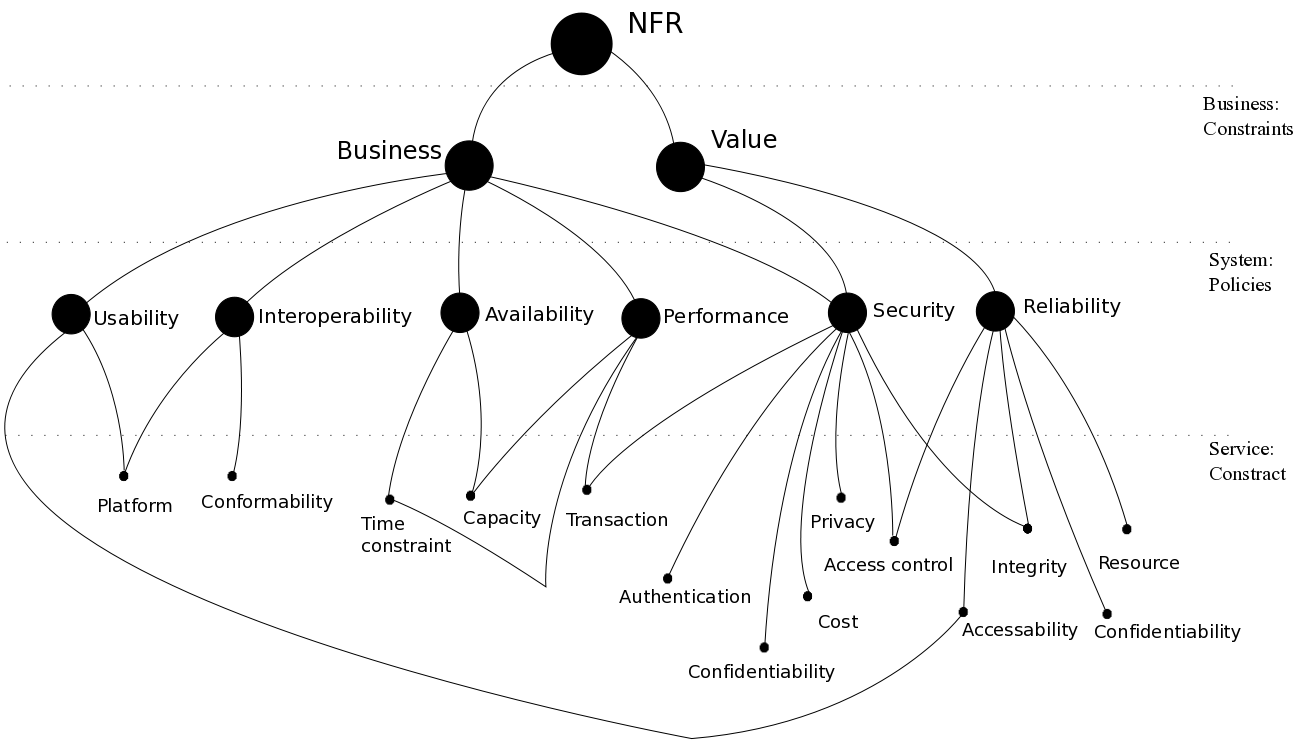
\includegraphics[width=0.90\textwidth]{figs/nfrRelationship.png}
\caption{Relationship between  NFR Concepts.}
\label{fig:nfr-relationship}   
\end{figure*}  


Chollet et al.~\cite{CholletL09} associate (non-functional) \textit{quality properties} to 
(functional) activities. The authors present a security meta-model for web service
composition. The NFRs considered are \textit{authentication}, \textit{integrity} and \textit{confidentiality}. Each NFR is associated with a service activity.


Ceri et al.\cite{CeriDMF07} uses the notions of \textit{policy}, \textit{rule}, \textit{condition} and \textit{action model} to specify NFRs.
Agarwal et al.~\cite{AgarwalLS09} associate \textit{service policies} to services. 
Each service may also have \textit{properties}, such as \textit{security} and \textit{reliability}. 
Ovaska et al.~\cite{OvaskaEHPA10} use the terms \textit{quality attribute}, \textit{category}, \textit{conceptual layer} and \textit{importance} to organize and classify NFRs.
Other authors do not define specific terms to refer to NFRs. 
They use terms such as \textit{attribute}~\cite{ZhangPSP05,BasinDL06,JeongCL09}, 
\textit{property}~\cite{Fabra2011}, 
\textit{factor}~\cite{MohantyRP10,GutierrezRF10}, 
\textit{characteristic}~\cite{DiamadopoulouMPS08}, 
\textit{quality level}~\cite{ModicaTV09}, and
\textit{value}~\cite{ThissenW06,BasinDL06}.


% The purpose of this analysis is to identify the properties and non-functional
% requirements used in the development of systems, looking for patterns
% or relationships between non-functional concepts in different
% modeling levels.

Despite of the different notations found in the literature for classifying NFRs, some non-functional requirements are frequently considered, such as \textit{security}, \textit{performance}, \textit{reliability}, \textit{usability}, and \textit{availability}.
However, distinct hierarchies and models are proposed for NFRs,  according to different points of view.
We have identified a number of approaches~\cite{DAmbrogio06,CholletL09,SchmelingCM11,BasinDL06,Fabra2011,OvaskaEHPA10} that use MDD (Model Driven Development) for designing and developing applications. 

%Although there exist many different types of notation used for classify
%non-functional requirements, in general, the values associated to them are the
%same, \textit{i.e.} \textit{security, performance, reliability, usability, availability}, etc. What
%distinguishes the different approaches is the adoption of different NFR
%hierarchies in order to prioritize or classify the quality requirements. 
%Another interesting factor
%is that the each work uses different approaches to model these requirements.
%Thus, there are different kinds of notations for non-functional
%requirements.



Fabra \textit{et al.}~\cite{Fabra2011} also describes the importance of  MDD for service-oriented applications. This work  presents a complete development methodology, although this methodology is not centered on NFRs.
The authors in~\cite{ThissenW06,ZhangPSP05} use formal methods to define a service-based development process that takes NFRs into account. 
In~\cite{AgarwalLS09,PastranaPK11} ontologies are used to define and model NFRs, 
whereas in~\cite{XiaoCZBOLH08,GutierrezRF10} Business Process Modeling (BPM) is used for
system specification, including NFRs. 
The majority of the authors concentrate on the  modeling of service compositions, although a significant number of approaches is focused on the definition of NFR models.


In the method defined in~\cite{XiaoCZBOLH08}, tasks in the process model can be 
annotated with \textit{non-functional attributes} (NFAs). 
NFAs are defined apart  and are concerned with data items or tasks. 
NFAs for data considers \textit{value} and \textit{range}, whereas NFAs for tasks include \textit{cost}, \textit{time}, \textit{resources} and \textit{expressions}.

The proposal in~\cite{ThissenW06} presents steps for  selecting services 
by taking QoS information into account. The proposed steps are: 
\textit{(i)} identification of relevant QoS information; 
\textit{(ii)} identification of basic composition patterns and 
QoS aggregation rules for these patterns; and 
\textit{(iii)} definition of a selection mechanism of services. 
The QoS properties considered are \textit{performance}, \textit{cost}, \textit{reliability} and
\textit{availability}. 
  
Karunamurthy et al.~\cite{Karunamurthy2012787} use the term \textit{non-function parameters} to define NFRs, such as \textit{cost}, \textit{response time}, \textit{availability}, \textit{security}, \textit{reliability} and \textit{reputation}.  
The \textit{Non-Func\-tion\-al Specification Language} (NFSL) is proposed as a domain specific language (DSL) to express \textit{non-function parameters}.

Liu et al.~\cite{Liu20121080} use the term \textit{QoS parameter} to describe non-functional requirements such as \textit{cost}, \textit{execution duration}, \textit{accuracy}, \textit{security}, \textit{integrity}, \textit{availability} and \textit{reliability}.  
In the same way, Tran et al.~\cite{Tran2012531} use the term \textit{QoS policies} to classify similar non-functional requirements.

Li et al.~\cite{Li2013} associate \textit{dimensions} to  \textit{QoS parameters} to classify NFRs.  
For instance, the \textit{time} dimension is associated to the \textit{execution time} and \textit{communication time} parameters; the \textit{spatial} dimension is associated to the \textit{storage capacity} and \textit{message length} parameters; the \textit{reliability} dimension is associated to the \textit{availability} and \textit{reliability} parameters and the \textit{cost} dimension is associated to the \textit{service cost} parameter.
Rumpel et al.~\cite{Rumpel2012}  associate \textit{quality requirements} to  \textit{quality properties}. Quality requirements are intended to be specified as constraints. 


\section{Classification of NFR}
\label{sec:classification}

Our systematic review is useful to identify those aspects of the NFR treatment in web service development that are consensual among authors.
These aspects include terminology to denote concepts as well as the relationships among them.

Most works agree on distinguishing three points of view, namely the point of view of the organization (or Business view), of the individual service providers (or Service view) and of the composition designer (or System view).
The Business view is concerned with the business logic (\textit{i.e.}, an abstract level of tasks, defined by the guidelines and constraints imposed by the organization).
Service and System views are concerned with the implementation of the software solution: The Service level is concerned with the building blocks of the application.
It may use web services provided by third party sources.
The System level is concerned with the coordination of services, to implement the business logic.

 


Table \ref{tab:result04} shows the NFR classification we propose, in accordance to these points of view.
The second column of the table presents the term we suggest for NFRs at each level.
The last column contains the most common terms found in the literature for specific classes of NFRs at each level.

\begin{table}[ht!]
\centering
%\scriptsize
\small
\begin{tabular}{l|l|l}
  \hline 
  \hline
   \textbf{\textit{Viewpoint}} & \textbf{\textit{Term}} & \textbf{\textit{Concepts}}  
   \\
  \hline
  \hline   
  Business View & Constraint  & Business Constraint,    
 \\  
  &   & Value Constraint\\
   \hline    
 
   &  & Security, Performance,\\ 
   & & Interoperability, Scalability,\\
  System View & Policy & Reliability, Usability,\\
   & & Transactional Behaviour,\\
   & & Availability \\ 
   \hline
     &  & Integrity, Transaction,  \\
   &  & Accessibility, Encryption, \\
   &  & Cost, Time Constraint, \\
  Service View & Contract & Encryption, Platform, \\
   &  & Privacy, Authentication, \\
   &  & Resource, Capacity, \\
   &  & Privacy, Confidentiability 
   \\   \hline
  \hline  
\end{tabular}
\caption{NFR Classification.}
\label{tab:result04}
\end{table} 

The relationship between concepts of the three levels is depicted in Figure~\ref{fig:nfr-relationship}.
The \textit{Contracts} bound to services should be devised to implement \textit{Policies} (at the System level).
These policies are used to guarantee business \textit{Constraints}.



Another classification of NFRs can be found in~\cite{Yeom2006}, which does not considers NFRs over data (but just over functions and service performance). 
We consider that it is important to classify the requirements of business and data (value) restrictions, since data processing is an essential part of the web service execution.

In the next subsection we present a NFR-centred meta-model for web service applications.

\begin{figure}[ht!]  
\centering  
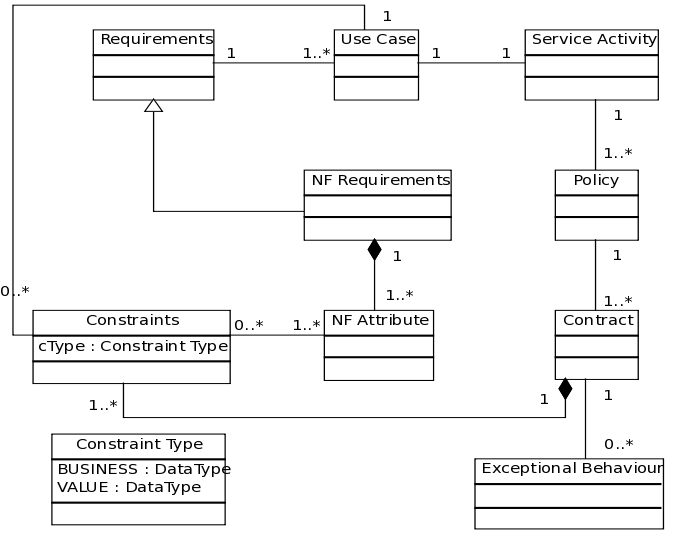
\includegraphics[width=0.9\textwidth]{figs/metamodelo.png}
\caption{NFR Model.}
\label{fig:NRFmodel} 
\end{figure} 


\subsection{NFR Meta-Model} 
\label{sec:nfr-metamodel}

The model presented in Figure~\ref{fig:NRFmodel} shows the relationship between
those concepts
we consider important for quality requirements used
in service-based development.

In this model, one \texttt{Requirement} (functional or non-func\-tion\-al) can be represented by one or more use cases. 
Each use case represents a \texttt{Service Activity}. 
Each use case has \textit{business} or
\textit{value} constraints. 
\textit{Business constraints} are restriction on functions and how they may be implemented. The \textit{value constraints} are restrictions on
the service interface, which the desired values for input and output data. Each
constraint is associated with NFAs.

A \texttt{Contract} is a set of constraints for the same function. For example,
a contract for the payment operation. The constraints for payment are: (i) the
value amount should not be less than 10 euros and (ii) the user should always
receive a purchase confirmation by phone message. This restrictions are
grouped into a single contract for payment verification. 

% These constraints
% are also associated with non-functional attributes, e.g., reliability,
% transactions and data privacy card.
 
An \texttt{Exceptional Behavior} happens when a contract is not respected. When
this happens a new function is called or the process is stopped. For example, if
the bank does not authorize the payment, the system offers alternative forms
of payment such as PayPal.

Finally a \texttt{Policy} groups similar contracts. For example, security
contracts are grouped into a security policy and performance contracts are
grouped into a performance policy.

\section{Conclusions}
\label{sec:conclusion}
 
 
Notice that \textit{security} and \textit{performance} are the most frequently considered NFRs.
\textit{Reliability} is also present in most proposals.

 
 
 

 
 
This paper presented a systematic review of NFRs associated with web services.
We grouped the NFRs according to their characteristics and analyzed them in each
context of application. 
We identified the main NFR concepts associated with service-based development. 
We also presented a synthesis of the most common concepts found in the literature. 
We suggest a characterization of NFR-related concepts and a classification by considering three points of view: \textit{business}, \textit{services} and \textit{system}. 

Our analysis and classification can help to improve the development of
service-based applications, by focusing on the guarantee of quality requirements. 

We believe that the specification of NFRs from the early stages of the software process
can improve the quality of the solution.
   
\bibliographystyle{plain}
\bibliography{biblio} 




\end{document}
